%%%%%%%%%%%%%%%%%%%%%%%%%%%%%%%%%%%%%%%%%%%%%%%%%%%%%%%%%%%%%%%

% Set up document

\documentclass{beamer}
\usecolortheme{whale}
\setbeamersize{text margin left=5mm,text margin right=5mm}

% Used to create a section slide between section
\AtBeginSection[]{
  \begin{frame}
  \vfill
  \centering
  \begin{beamercolorbox}[sep=8pt,center,shadow=true,rounded=true]{title}
    \usebeamerfont{title}\insertsectionhead\par%
  \end{beamercolorbox}
  \vfill
  \end{frame}
}

% Remove default navigation symbols and add just  page number
\setbeamertemplate{navigation symbols}{} % Clear default navigation
\addtobeamertemplate{navigation symbols}{}{%
    \usebeamerfont{footline}%
    \usebeamercolor[fg]{footline}%
    \hspace{1em}%
    \insertframenumber/\inserttotalframenumber
}


%%%%%%%%%%%%%%%%%%%%%%%%%%%%%%%%%%%%%%%%%%%%%%%%%%%%%%%%%%%%%%%

% Title page

\title{Stroke Audit Machine Learning (SAMueL) \\ Workshop 1}
\subtitle{Investigating variation in clinical decision-making with explainable AI}


\author{Kerry Pearn\inst{1}, Michael Allen\inst{1}, Keira Pratt-Boyden\inst{1}, Martin James\inst{1,2} }
\institute{\inst{1} University of Exeter Medical School \inst{2} Royal Devon University Healthcare NHS Foundation Trust}

%\institute{Overleaf}
\date{November 2022}


\begin{document}

\frame{\titlepage}

%%%%%%%%%%%%%%%%%%%%%%%%%%%%%%%%%%%%%%%%%%%%%%%%%%%%%%%%%%%%%%%

\begin{frame}
\frametitle{Breaking down the emergency stroke pathway into key steps}
\begin{center}
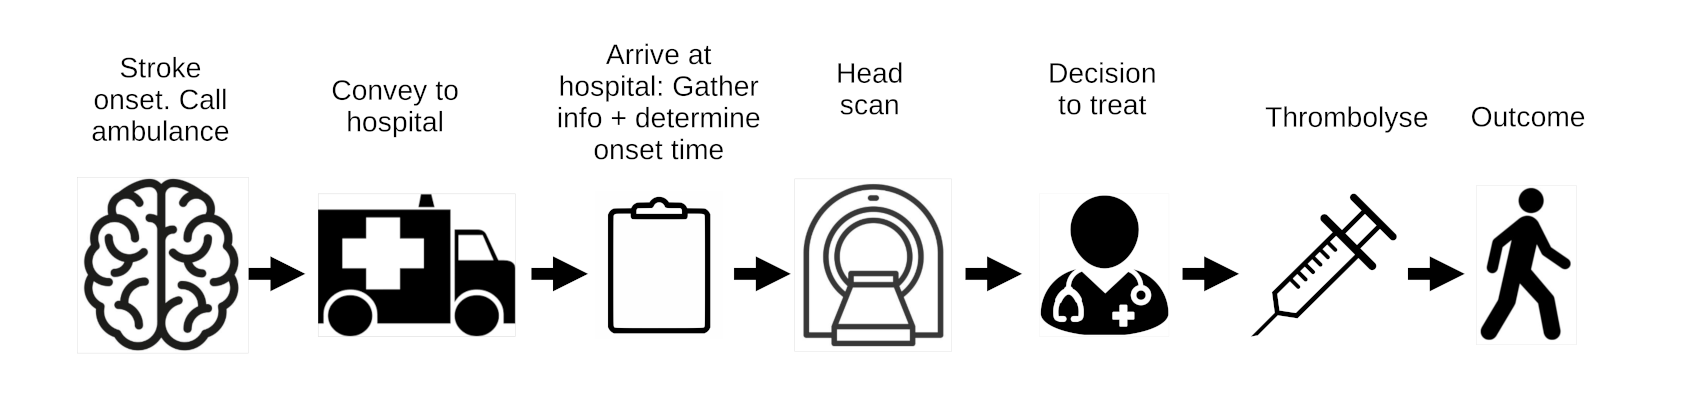
\includegraphics[width=1.0\textwidth]{./images/pathway}
\end{center}
We can model key changes to pathway:
\begin{itemize}
    \item What if the pathway were faster?
    \item What if hospital determined the stroke onset time in more patients?
    \item What if clinical decision-making was like that of \emph{benchmark} hospitals? (Predict what treatment a patient would receive at other hospitals).
\end{itemize}
\end{frame}

%%%%%%%%%%%%%%%%%%%%%%%%%%%%%%%%%%%%%%%%%%%%%%%%%%%%%%%%%%%%%%%

\begin{frame}
\frametitle{Machine learning overview}
\begin{center}
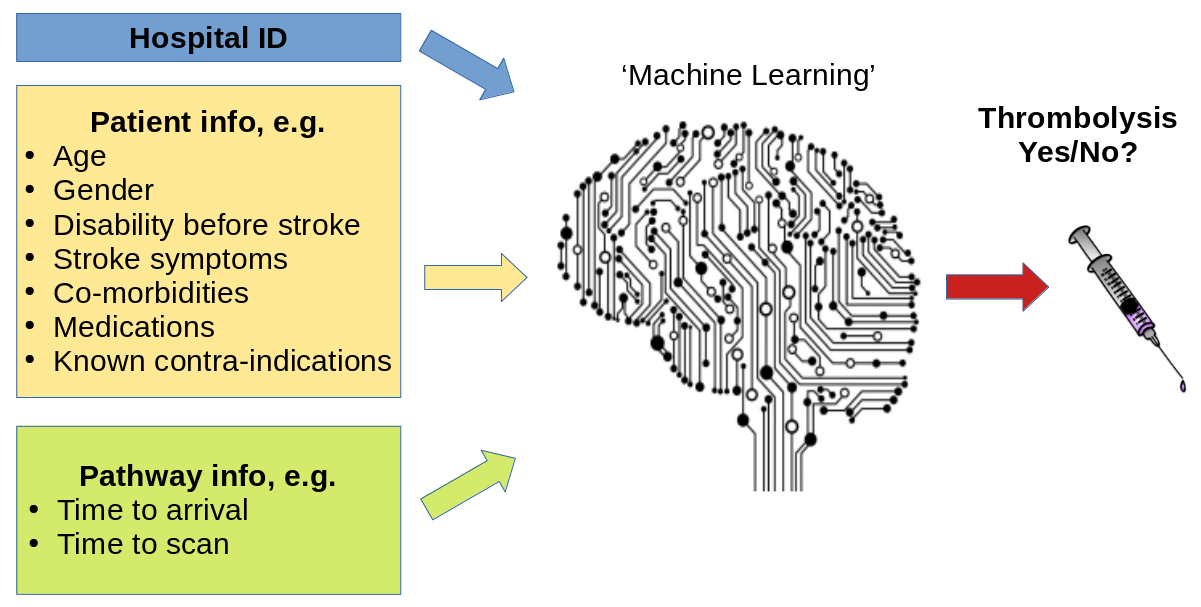
\includegraphics[width=0.95\textwidth]{./images/ml_model_high_level}
\end{center}

We accessed 240,000 emergency stroke admissions in England and Wales over three years.
\end{frame}

%%%%%%%%%%%%%%%%%%%%%%%%%%%%%%%%%%%%%%%%%%%%%%%%%%%%%%%%%%%%%%%

\begin{frame}{Model accuracy, and simplification}

Our machine learning models use XGBoost classification, and are based on all patients who arrive within 4 hours of known stroke onset.

\vspace{5mm}

\begin{columns}

    \begin{column}{0.5\textwidth}
    
        The full model has 61 patient features:
        
        \begin{footnotesize}
        \begin{itemize}
            \item Overall accuracy = 85.2\%
            \item Best combined sensitivity and specificity = 84.3\%
            \item ROC AUC = 0.921
        \end{itemize}
        \end{footnotesize}
        
        \vspace{3mm}
        
        A simplified model with 8 features
        
        \begin{footnotesize}
        \begin{itemize}
            \item Overall accuracy = 84.8\%
            \item Best combined sensitivity and specificity = 83.8\%
            \item ROC AUC = 0.916
        \end{itemize}
        \end{footnotesize}
    
    \end{column}
    
    \begin{column}{0.5\textwidth}
    The 8 features of the simplified model are:
        \begin{footnotesize}
        \begin{enumerate}
            \item Arrival-to-scan time
            \item Stroke type (infarction/haemorrhage)
            \item Stroke severity (NIHSS)
            \item Precise or estimated stroke onset time
            \item Prior disability level (mRS)
            \item Stroke team
            \item Use of AF anticoagulants
            \item Onset-to-arrival time
        \end{enumerate}
        \end{footnotesize}
        
    \vspace{2mm}
    \tiny{There are only very weak correlations between the selected features with no R-squared being greater than 0.05.}
    \end{column}
    





\end{columns}


    
\end{frame}


%%%%%%%%%%%%%%%%%%%%%%%%%%%%%%%%%%%%%%%%%%%%%%%%%%%%%%%%%%%%%%%

\begin{frame}
\frametitle{Explaining model predictions with SHAP values}

SHAP values show the influence of features (even for \emph{`black box'} models).

\begin{center}
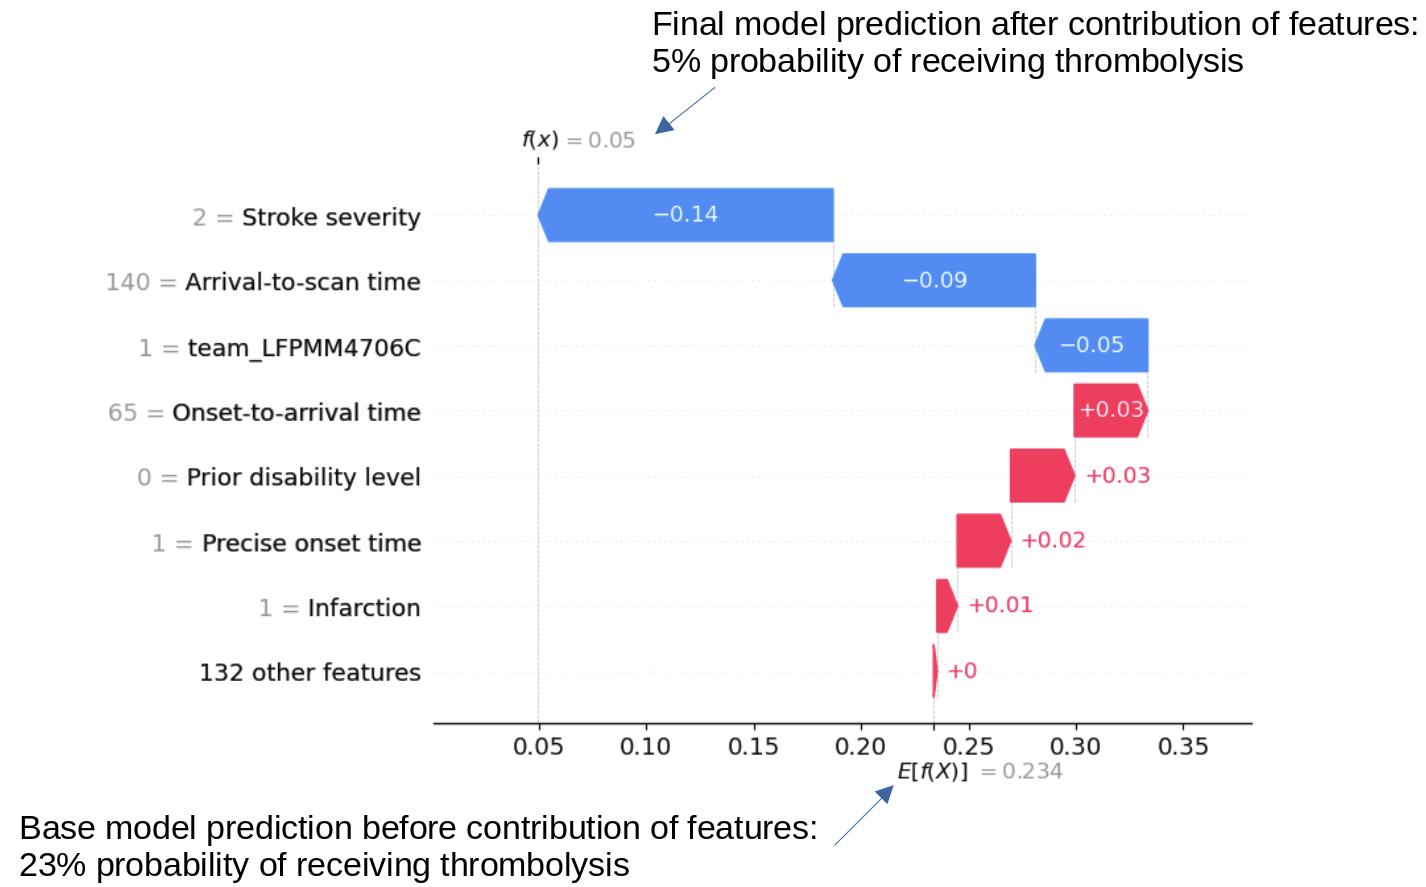
\includegraphics[width=0.85\textwidth]{./images/xgb_waterfall_low_probability.jpg}
\end{center}
\end{frame}


%%%%%%%%%%%%%%%%%%%%%%%%%%%%%%%%%%%%%%%%%%%%%%%%%%%%%%%%%%%%%%%

\begin{frame}
\frametitle{What drives use of thrombolysis across all hospitals?}

\footnotesize{Note: SHAP values here are \emph{log odds}. Each step-change in value of \textpm 1 changes the chances of receiving thrombolysis about 3-fold. (Plots are in order of feature importance.)}

\begin{center}
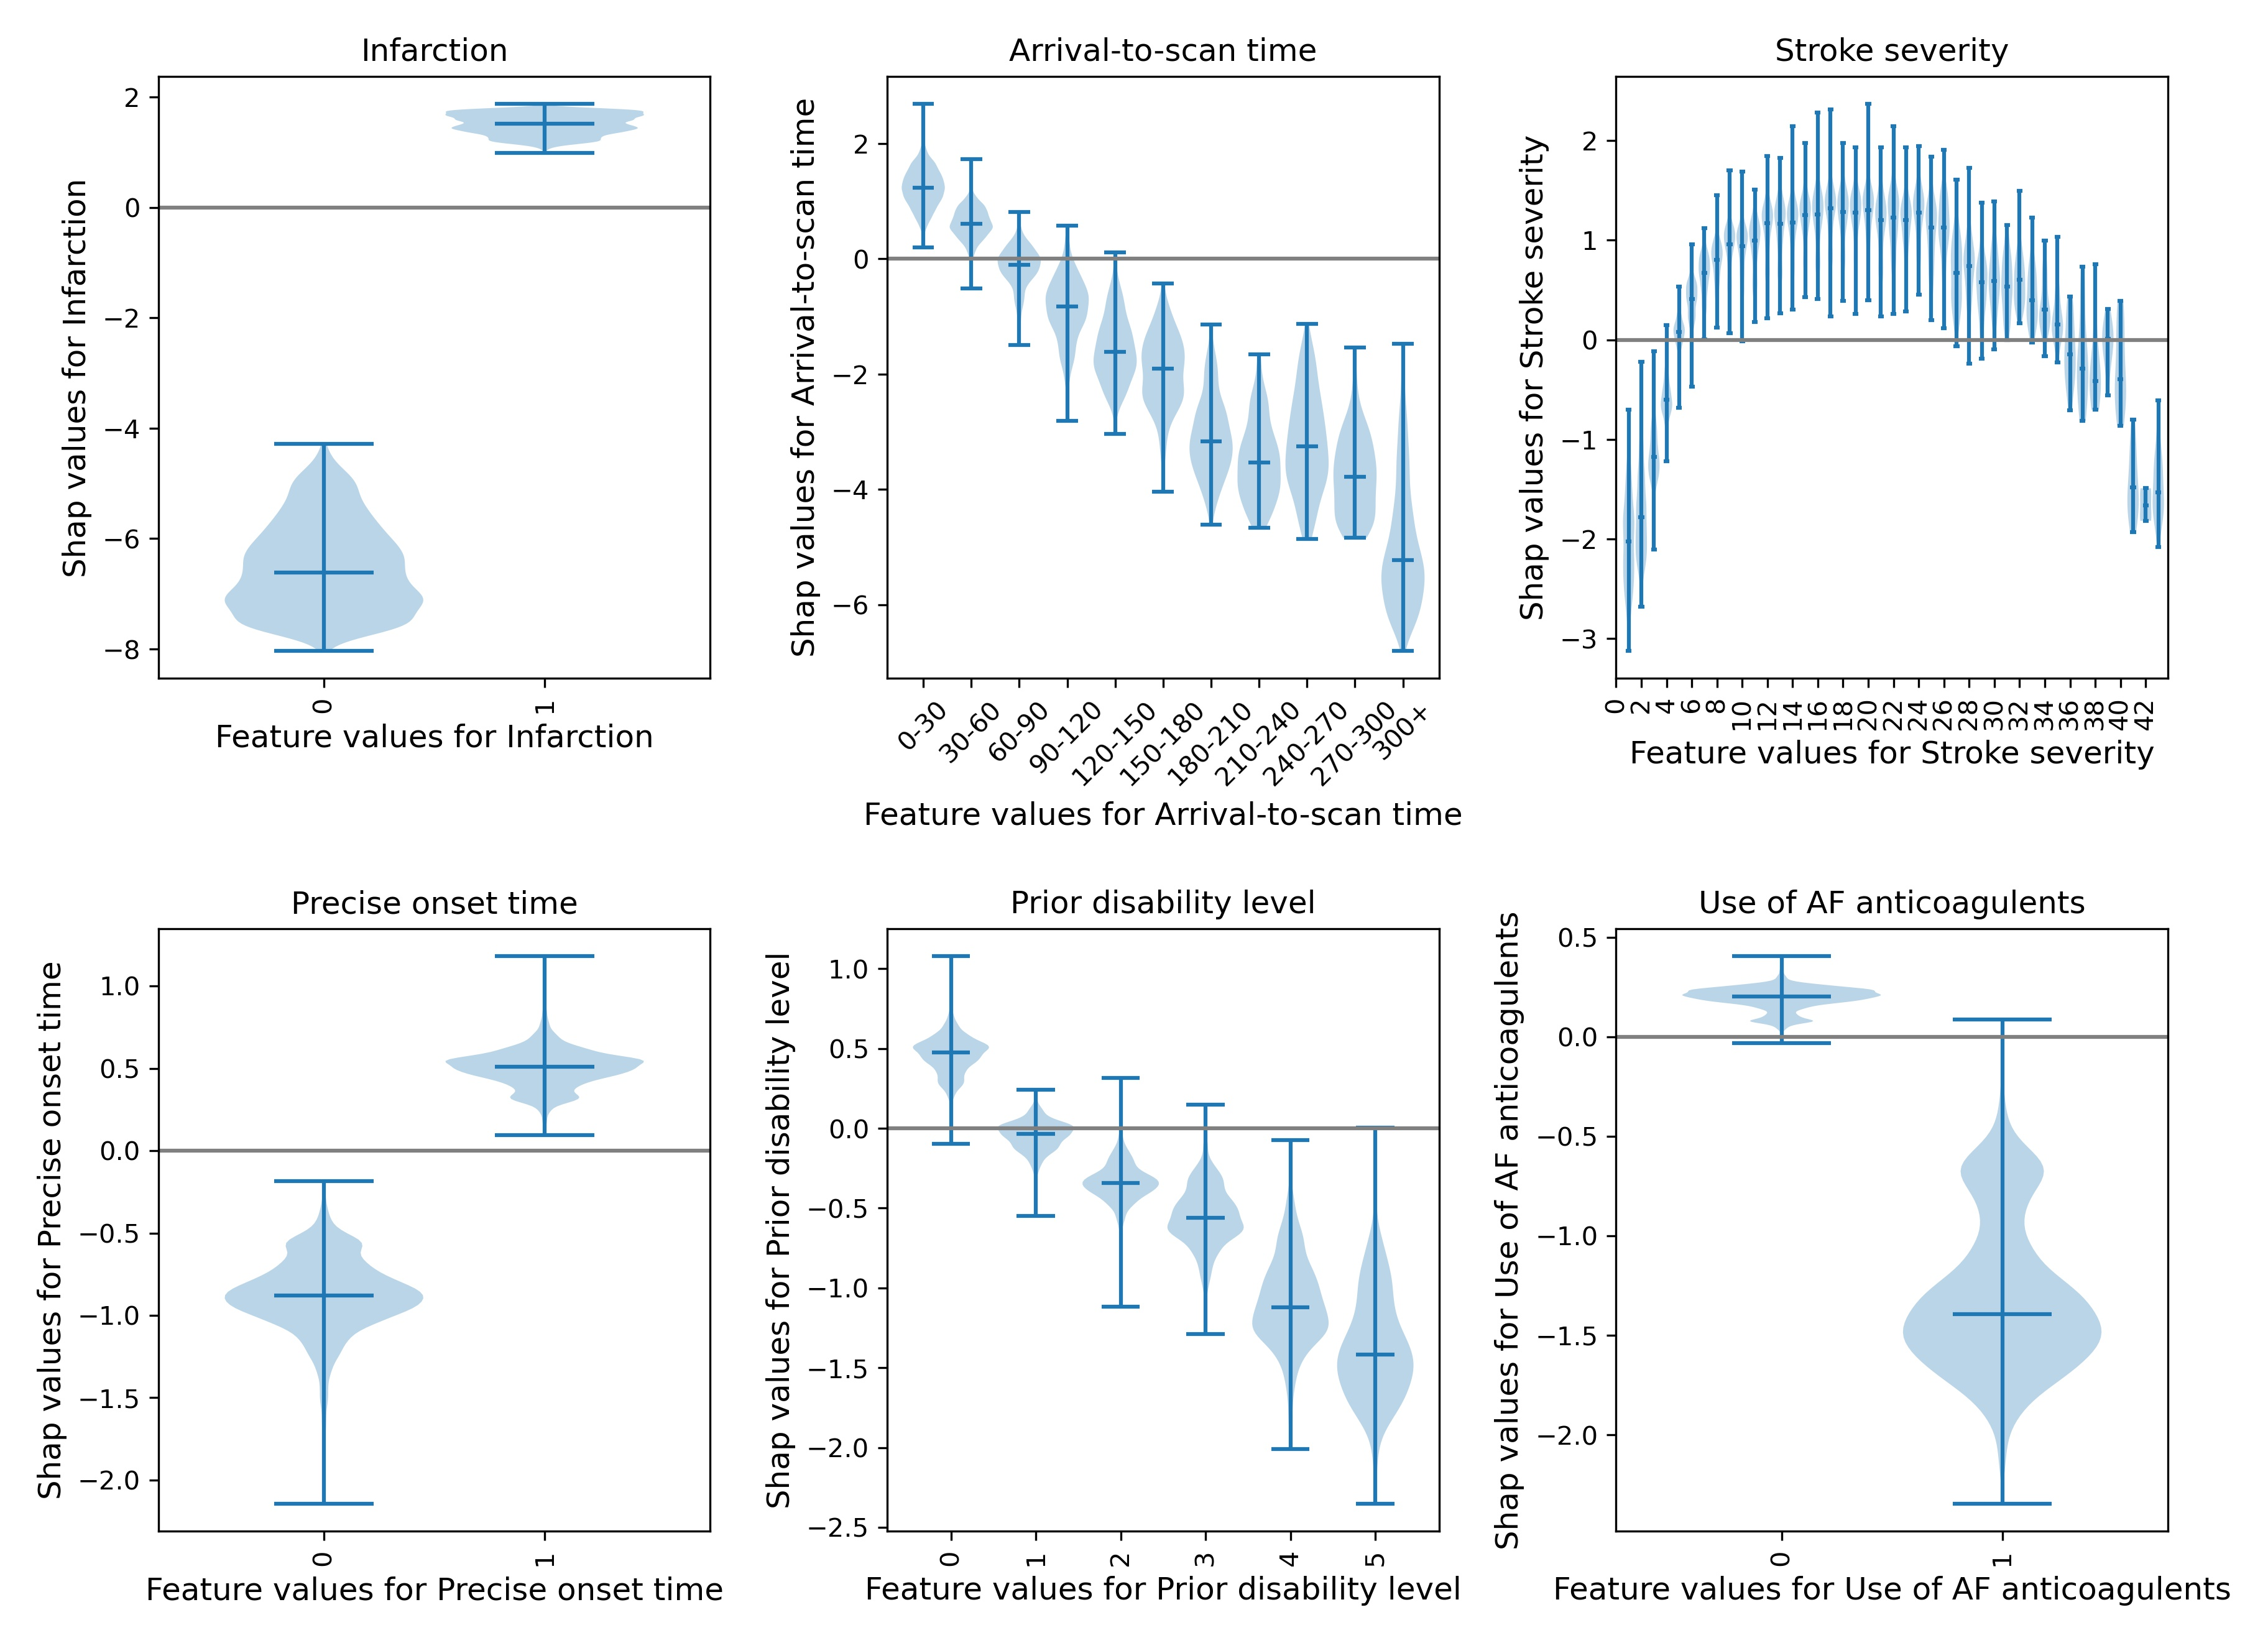
\includegraphics[width=0.80\textwidth]{./images/xgb_thrombolysis_shap_violin.jpg}
\end{center}
\end{frame}

%%%%%%%%%%%%%%%%%%%%%%%%%%%%%%%%%%%%%%%%%%%%%%%%%%%%%%%%%%%%%%%

\begin{frame}
\frametitle{Investigating how hospitals differ in thrombolysis decision-making (Patient 1: Base patient)}

Assuming there are no reasons not stated here to exclude a patient from use of thrombolysis, would you give this patient thrombolysis?

\vspace{3mm}

\begin{columns}
    \begin{column}{0.6\textwidth}
        \begin{itemize}
            \item Onset to arrival = 80 mins
            \item Arrival to scan = 20 mins
            \item Infarction = Yes
            \item NIHSS = 15
            \item Prior disability level = 0
            \item Precise onset time = Yes
            \item Use of AF anticoagulents = No
        \end{itemize}
    \end{column}
    
    \begin{column}{0.4\textwidth}
    
    \end{column}

\end{columns}
\end{frame}


\begin{frame}
\frametitle{Investigating how hospitals differ in thrombolysis decision-making (Patient 1: Base patient)}

Assuming there are no reasons not stated here to exclude a patient from use of thrombolysis, would you give this patient thrombolysis?

\vspace{3mm}

\begin{columns}
    \begin{column}{0.5\textwidth}
        \begin{itemize}
            \item Onset to arrival = 80 mins
            \item Arrival to scan = 20 mins
            \item Infarction = Yes
            \item NIHSS = 15
            \item Prior disability level = 0
            \item Precise onset time = Yes
            \item Use of AF anticoagulents = No
        \end{itemize}
    \end{column}
    
    \begin{column}{0.4\textwidth}
    Our model predicts 131 out of 132 (99\%) hospitals would give this patient thrombolysis.
    \end{column}

\end{columns}
\end{frame}

%%%%%%%%%%%%%%%%%%%%%%%%%%%%%%%%%%%%%%%%%%%%%%%%%%%%%%%%%%%%%%%

\begin{frame}
\frametitle{Investigating how hospitals differ in thrombolysis decision-making (Patient 2: Milder stroke)}

Assuming there are no reasons not stated here to exclude a patient from use of thrombolysis, would you give this patient thrombolysis?

\vspace{3mm}

\begin{columns}
    \begin{column}{0.6\textwidth}
        \begin{itemize}
            \item Onset to arrival = 80 mins
            \item Arrival to scan = 20 mins
            \item Infarction = Yes
            \item \emph{NIHSS = 5}
            \item Prior disability level = 0
            \item Precise onset time = Yes
            \item Use of AF anticoagulents = No
        \end{itemize}
    \end{column}
    
    \begin{column}{0.4\textwidth}
    
    \end{column}

\end{columns}
\end{frame}


\begin{frame}
\frametitle{Investigating how hospitals differ in thrombolysis decision-making (Patient 2: Milder stroke)}

Assuming there are no reasons not stated here to exclude a patient from use of thrombolysis, would you give this patient thrombolysis?

\vspace{3mm}

\begin{columns}
    \begin{column}{0.5\textwidth}
        \begin{itemize}
            \item Onset to arrival = 80 mins
            \item Arrival to scan = 20 mins
            \item Infarction = Yes
            \item \emph{NIHSS = 5}
            \item Prior disability level = 0
            \item Precise onset time = Yes
            \item Use of AF anticoagulents = No
        \end{itemize}
    \end{column}
    
    \begin{column}{0.4\textwidth}
    Our model predicts 120 out of 132 (91\%) hospitals would give this patient thrombolysis.
    \end{column}

\end{columns}
\end{frame}

%%%%%%%%%%%%%%%%%%%%%%%%%%%%%%%%%%%%%%%%%%%%%%%%%%%%%%%%%%%%%%%

\begin{frame}
\frametitle{Investigating how hospitals differ in thrombolysis decision-making (Patient 3: Some pre-stroke disability)}

Assuming there are no reasons not stated here to exclude a patient from use of thrombolysis, would you give this patient thrombolysis?

\vspace{3mm}

\begin{columns}
    \begin{column}{0.6\textwidth}
        \begin{itemize}
            \item Onset to arrival = 80 mins
            \item Arrival to scan = 20 mins
            \item Infarction = Yes
            \item NIHSS = 15
            \item \emph{Prior disability level = 2}
            \item Precise onset time = Yes
            \item Use of AF anticoagulents = No
        \end{itemize}
    \end{column}
    
    \begin{column}{0.4\textwidth}
    
    \end{column}

\end{columns}
\end{frame}

%%%%%%%%%%%%%%%%%%%%%%%%%%%%%%%%%%%%%%%%%%%%%%%%%%%%%%%%%%%%%%%

\begin{frame}
\frametitle{Investigating how hospitals differ in thrombolysis decision-making (Patient 3: Some pre-stroke disability)}

Assuming there are no reasons not stated here to exclude a patient from use of thrombolysis, would you give this patient thrombolysis?

\vspace{3mm}

\begin{columns}
    \begin{column}{0.5\textwidth}
        \begin{itemize}
            \item Onset to arrival = 80 mins
            \item Arrival to scan = 20 mins
            \item Infarction = Yes
            \item NIHSS = 15
            \item \emph{Prior disability level = 2}
            \item Precise onset time = Yes
            \item Use of AF anticoagulents = No
        \end{itemize}
    \end{column}
    
    \begin{column}{0.4\textwidth}
    Our model predicts 126 out of 132 (96\%) hospitals would give this patient thrombolysis.
    \end{column}

\end{columns}
\end{frame}

%%%%%%%%%%%%%%%%%%%%%%%%%%%%%%%%%%%%%%%%%%%%%%%%%%%%%%%%%%%%%%%

\begin{frame}
\frametitle{Investigating how hospitals differ in thrombolysis decision-making (Patient 4: Estimated stroke onset time)}

Assuming there are no reasons not stated here to exclude a patient from use of thrombolysis, would you give this patient thrombolysis?

\vspace{3mm}

\begin{columns}
    \begin{column}{0.6\textwidth}
        \begin{itemize}
            \item Onset to arrival = 80 mins
            \item Arrival to scan = 20 mins
            \item Infarction = Yes
            \item NIHSS = 15
            \item Prior disability level = 0
            \item \emph{Precise onset time = No}
            \item Use of AF anticoagulents = No
        \end{itemize}
    \end{column}
    
    \begin{column}{0.4\textwidth}
    
    \end{column}

\end{columns}
\end{frame}


\begin{frame}
\frametitle{Investigating how hospitals differ in thrombolysis decision-making (Patient 4: Estimated stroke onset time)}

Assuming there are no reasons not stated here to exclude a patient from use of thrombolysis, would you give this patient thrombolysis?

\vspace{3mm}

\begin{columns}
    \begin{column}{0.5\textwidth}
        \begin{itemize}
            \item Onset to arrival = 80 mins
            \item Arrival to scan = 20 mins
            \item Infarction = Yes
            \item NIHSS = 15
            \item Prior disability level = 0
            \item \emph{Precise onset time = No}
            \item Use of AF anticoagulents = No
        \end{itemize}
    \end{column}
    
    \begin{column}{0.4\textwidth}
    Our model predicts 84 out of 132 (64\%) hospitals would give this patient thrombolysis.
    \end{column}

\end{columns}
\end{frame}

%%%%%%%%%%%%%%%%%%%%%%%%%%%%%%%%%%%%%%%%%%%%%%%%%%%%%%%%%%%%%%%

\begin{frame}
\frametitle{Investigating how hospitals differ in thrombolysis decision-making (Patient 5: Combined changes)}

Assuming there are no reasons not stated here to exclude a patient from use of thrombolysis, would you give this patient thrombolysis?

\vspace{3mm}

\begin{columns}
    \begin{column}{0.6\textwidth}
        \begin{itemize}
            \item Onset to arrival = 80 mins
            \item Arrival to scan = 20 mins
            \item Infarction = Yes
            \item \emph{NIHSS = 5}
            \item \emph{Prior disability level = 2}
            \item \emph{Precise onset time = No}
            \item Use of AF anticoagulents = No
        \end{itemize}
    \end{column}
    
    \begin{column}{0.4\textwidth}
    
    \end{column}

\end{columns}
\end{frame}


\begin{frame}
\frametitle{Investigating how hospitals differ in thrombolysis decision-making (Patient 5: Combined changes)}

Assuming there are no reasons not stated here to exclude a patient from use of thrombolysis, would you give this patient thrombolysis?

\vspace{3mm}

\begin{columns}
    \begin{column}{0.5\textwidth}
        \begin{itemize}
            \item Onset to arrival = 80 mins
            \item Arrival to scan = 20 mins
            \item Infarction = Yes
            \item \emph{NIHSS = 5}
            \item \emph{Prior disability level = 2}
            \item \emph{Precise onset time = No}
            \item Use of AF anticoagulents = No
        \end{itemize}
    \end{column}
    
    \begin{column}{0.4\textwidth}
    Our model predicts 3 out of 132 (2.3\%) hospitals would give this patient thrombolysis.
    \end{column}

\end{columns}
\end{frame}




%%%%%%%%%%%%%%%%%%%%%%%%%%%%%%%%%%%%%%%%%%%%%%%%%%%%%%%%%%%%%%%
\begin{frame}
\frametitle{Key findings}
General observations about thrombolysis use: The chance of receiving thrombolysis is increased by:
\emph{
\begin{itemize}
    \item Shorter arrival-to-scan times
    \item Mid-level stroke severity
    \item Precise onset time
    \item Lower pre-stroke disability
\end{itemize}
}

\vspace{5mm}

Lower thrombolysing units are particularly less likely to give thrombolysis to patients with:
\emph{
\begin{itemize}
    \item Low or high stroke severity
    \item Higher pre-stroke disability
    \item Estimated onset time
\end{itemize}
}

\end{frame}

%%%%%%%%%%%%%%%%%%%%%%%%%%%%%%%%%%%%%%%%%%%%%%%%%%%%%%%%%%%%%%%
\begin{frame}
\frametitle{Possible questions for discussion}

\begin{itemize}
    \item Does anything surprise you here?
    \item What are your attitudes to mild strokes and patients with estimated stroke-onset times?
    \item What might you do with the knowledge that different hospitals have different attitudes to mild strokes and patients with estimated stroke-onset times?
    \item Why do you think pre-stroke disability appears influential in thrombolysis decision-making?
\end{itemize}

\end{frame}


% EXTRA SLIDE(S)

%%%%%%%%%%%%%%%%%%%%%%%%%%%%%%%%%%%%%%%%%%%%%%%%%%%%%%%%%%%%%%%%%

\begin{frame}
\frametitle{When will low thrombolysing units not use thrombolysis when higher thrombolysing would?}

\footnotesize{Here, a high SHAP shows when a low-thrombolysing unit will reject use of thrombolysis when a higher thrombolysing hospital would use thrombolysis. (Plots are in order of feature importance.)}

\begin{center}
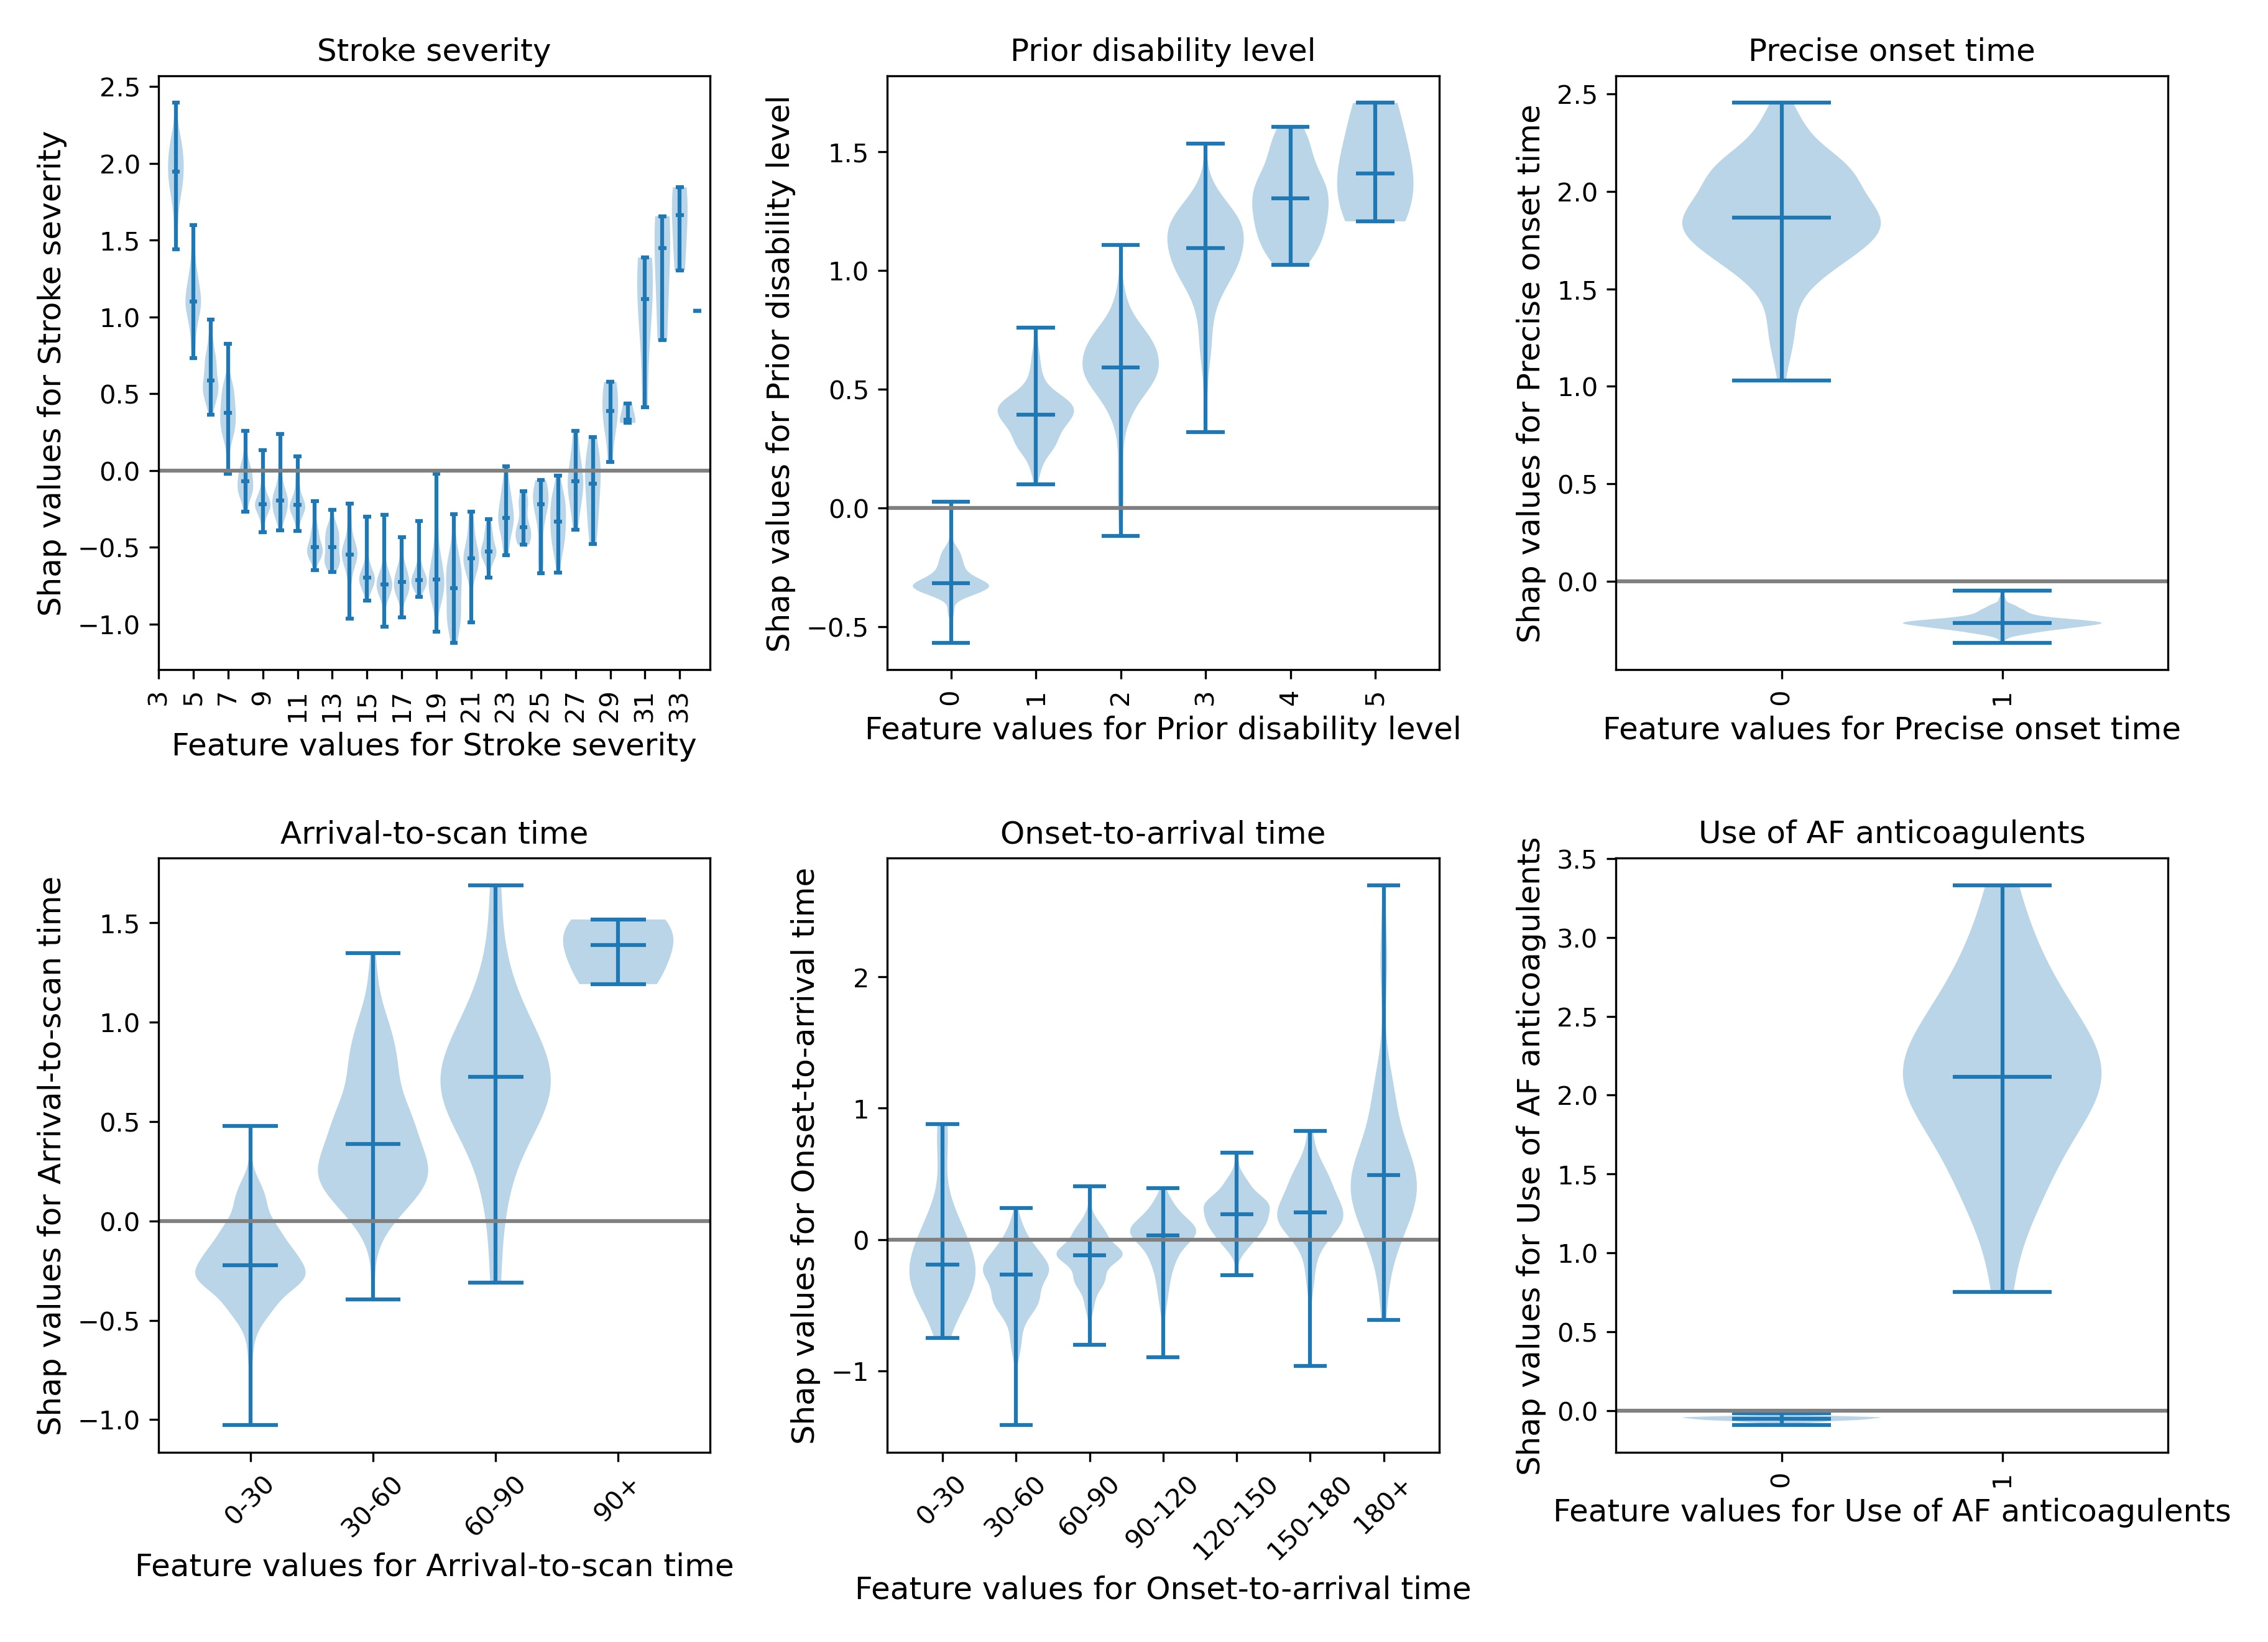
\includegraphics[width=0.75\textwidth]{./images/xgb_predicting_difference_shap_violin.jpg}
\end{center}
\end{frame}



\end{document}




